\documentclass[a4paper]{article}
\usepackage[utf8]{vietnam}
\usepackage{scrextend}
\usepackage{graphicx}
\usepackage{times}
\usepackage{hyperref}
\usepackage{enumitem}

\begin{document}

\section*{Câu 3. THỰC HÀNH}	
Chọn một ứng dụng trong thực tế và cho biết:

\begin{enumerate} 
	\item Miền tri thức. 
	\item Đối tượng sử dụng. 
	\item Yêu cầu và chức năng của hệ thống đòi hỏi vận dụng tri thức. 
	\item Phân tích và nhận định về đặc trưng của tri thức trong ứng dụng
\end{enumerate}


\section*{BÀI LÀM}
\textbf{QuickMath}\footnote{\url{https://quickmath.com/}} là một ứng dụng cung cấp lời giải theo từng bước cho các bài toán, từ đại số, giải phương trình cho đến giải tích, ma trận. Ngoài ra, ứng dụng này còn có thể hiển thị đồ thị của hàm số.

\subsection* {1. Miền tri thức}
Miền tri thức của \textbf{QuickMath} bao gồm tri thức đại số, giải tích, đại số tuyến tính.

\subsection*{2. Đối tượng sử dụng}
Đối tượng sử dụng bao gồm học sinh, sinh viên ở các cấp học, từ trung học cơ sở, trung~học phổ thông đến cao đẳng, đại học, và những người có nhu cầu tìm hiểu, giải các bài toán dạng công thức, ký hiệu (không phải dạng toán bằng lời văn).

\subsection*{3. Yêu cầu và chức năng của hệ thống đòi hỏi vận dụng tri thức}
\begin{itemize}
	\item \textbf{Yêu cầu: }Thiết bị điện tử dùng nhập yêu cầu (điện thoại, bàn phím máy tính), màn hình, kết nối mạng internet. Hệ thống yêu cầu người dùng nhập các bài toán dạng công thức, chọn đúng dạng đề mà người dùng cần giải (phương trình, hệ phương trình hay rút gọn đa thức, tính đạo hàm, ...)
	\begin{figure}
		\centering
		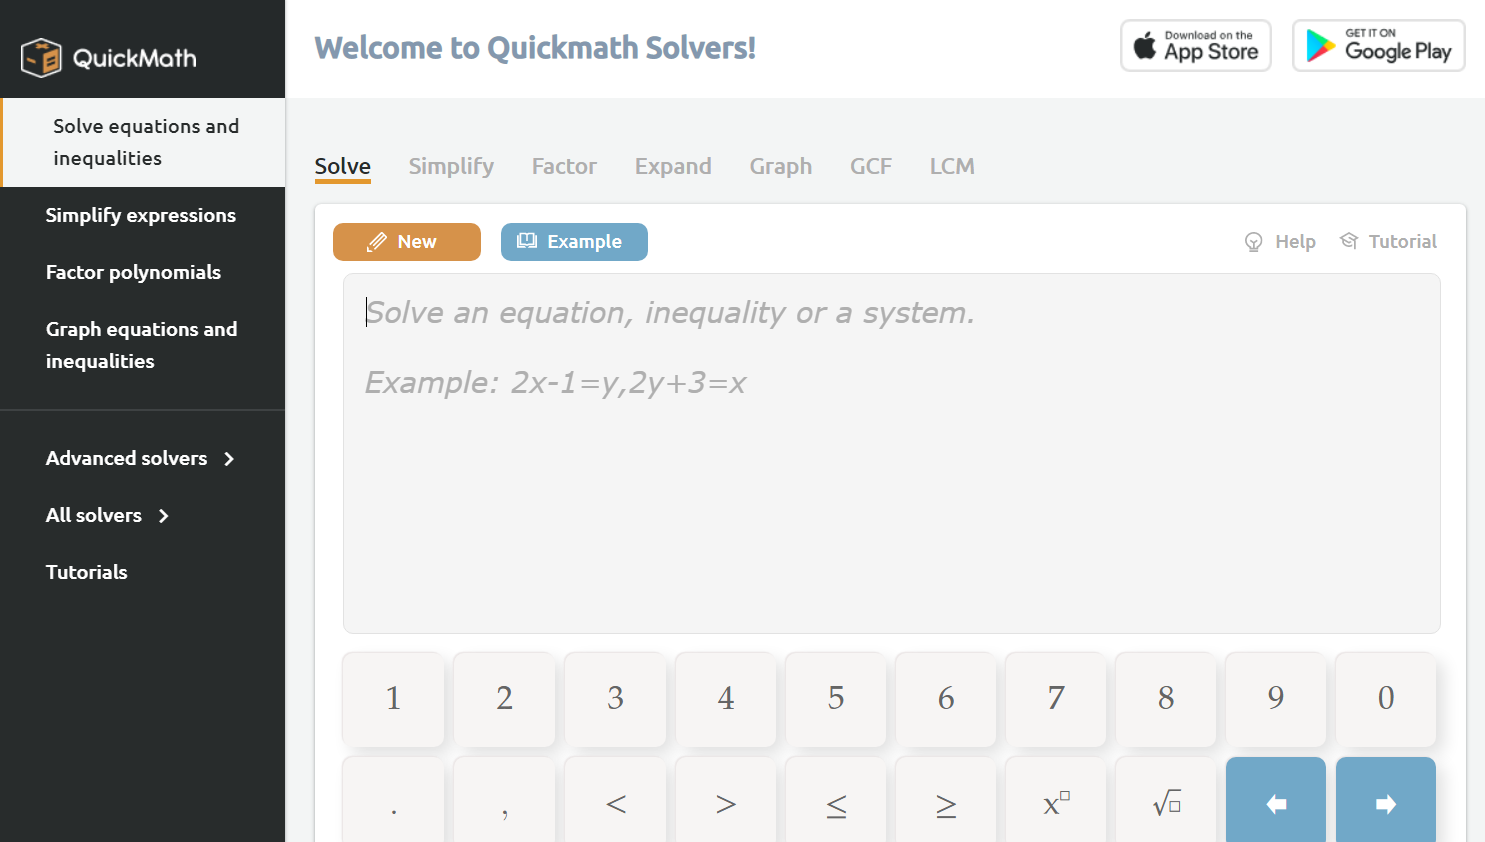
\includegraphics[width=0.7\linewidth]{quickmath1}
		\caption{Giao diện QuickMath và các tính năng}
		\label{fig:quickmath1}
	\end{figure}
	\item \textbf{Chức năng: } Nhận yêu cầu từ người dùng, sử dụng hệ thống tri thức trong ứng dụng để tính toán, biến đổi và trả ra màn hình kết quả với độ chính xác cao, lời giải chi tiết theo từng bước và thời gian xử lý là ngắn nhất. Ngoài ra, ở cuối mỗi dạng bài, \textbf{QuickMath} còn cung cấp cơ sở lý thuyết và các ví dụ để giải dạng bài đó.
	\begin{figure}
		\centering
		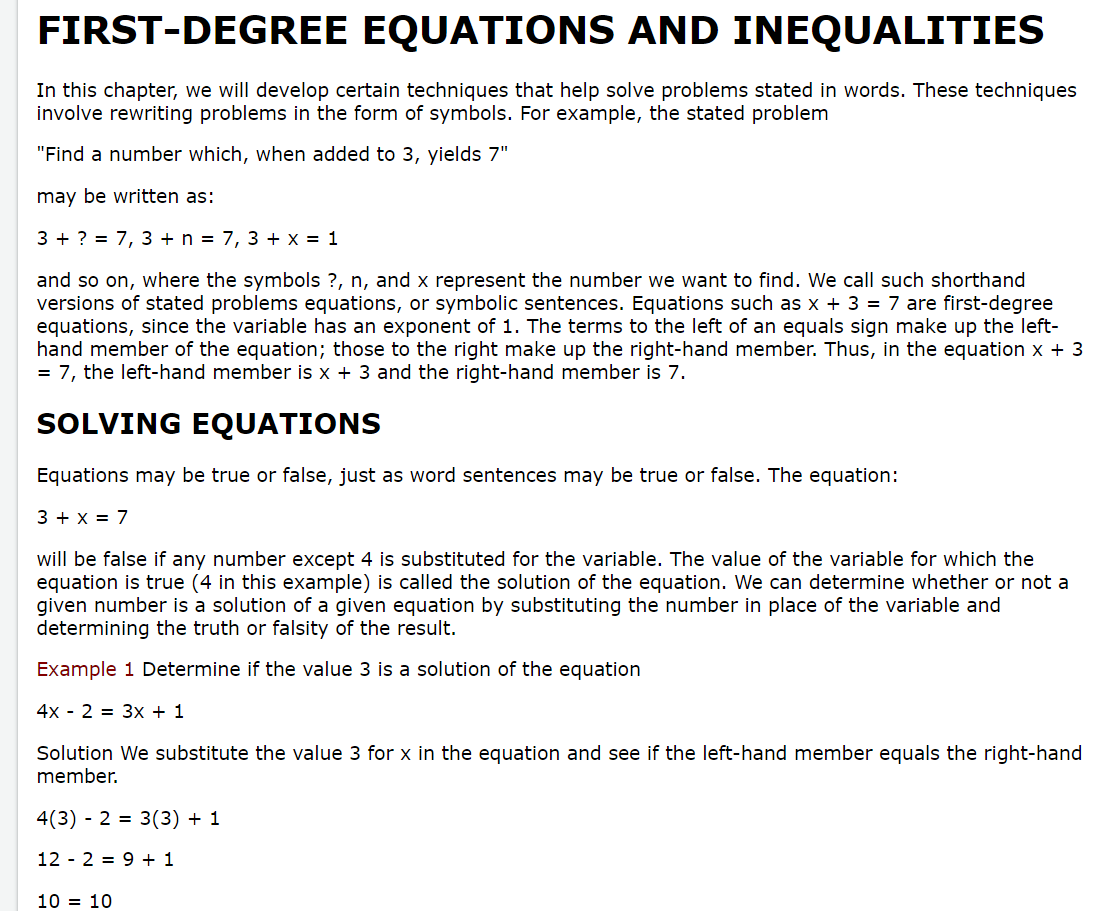
\includegraphics[width=0.7\linewidth]{quickmath3}
		\caption{Lý thuyết và ví dụ dưới mỗi tính năng tương ứng}
		\label{fig:quickmath3}
	\end{figure}
\end{itemize}


 \subsection*{4. Phân tích và nhận định về đặc trưng của tri thức trong ứng dụng}

\begin{enumerate}
\item [4.1] Phân tích đặc trưng của tri thức
\begin{itemize}
\item Tri thức về đại số bao gồm các phép toán số học, giải phương trình, bất phương trình, các phép tính liên quan đến đa thức: chia đa thức, phân tích tìm thừa số chung ... 
\item Tri thức về giải tích bao gồm các phép toán tính đạo hàm, vi phân, tích phân.
\item Tri thức về ma trận bao gồm các phép toán (cộng, trừ, nhân, chia) trên ma~trận), tìm ma trận nghịch đảo, tính định thức của ma trận.
\end{itemize}

\item [4.2]Nhận định về đặc trưng của tri thức
\begin{itemize}
\item \textbf{QuickMath} áp dụng từng bước giải theo hệ tri thức được đưa vào. Ví dụ, khi áp dụng tri thức về giải phương trình, việc "chuyển vế đổi dấu" chính là tri thức cộng vào hai vế của phương trình cho cùng một lượng. Điều này làm cho những lời giải của \textbf{QuickMath} có một số bước "dư thừa" trong tính toán, dù mô phỏng đúng cơ sở lý thuyết nhưng khác với thực tế làm bài của học sinh. 
\begin{figure}
	\centering
	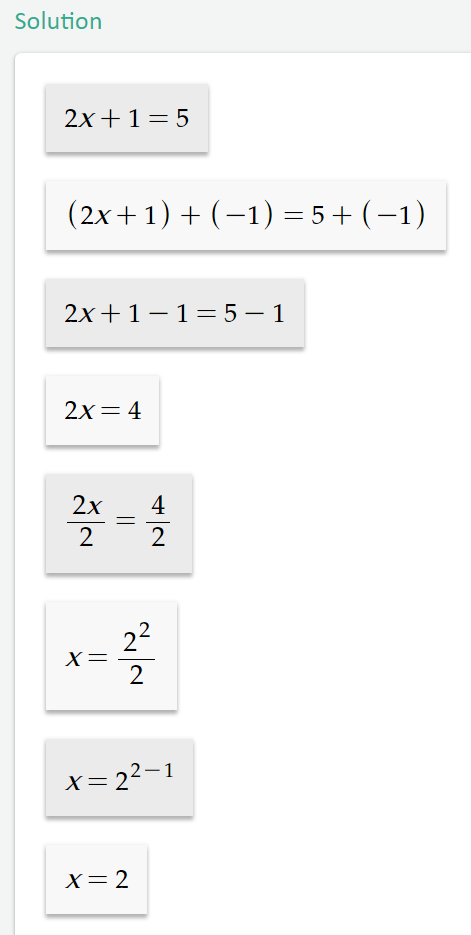
\includegraphics[width=0.7\linewidth]{quickmath2}
	\caption{Kết quả trả về khi giải phương trình bằng \textbf{QuickMath}}
	\label{fig:quickmath2}
\end{figure}
\item Các tri thức về đại số tuyến tính trong \textbf{QuickMath} nằm ở mức độ cơ bản, nằm riêng lẻ với các tri thức về hệ phương trình. Hệ phương trình trong \textbf{QuickMath} được giải chủ yếu bằng phương pháp biến đổi đại số (thêm bớt hạng tử) - phù hợp với tri thức học sinh trung học.
\item Tri thức về giải phương trình, cụ thể là phương trình bậc hai, được xây dựng dựa trên các phép biến đổi đại số (đặt nhân tử chung) và phương pháp tính bằng công thức nghiệm ($\Delta$)
\begin{figure}
	\centering
	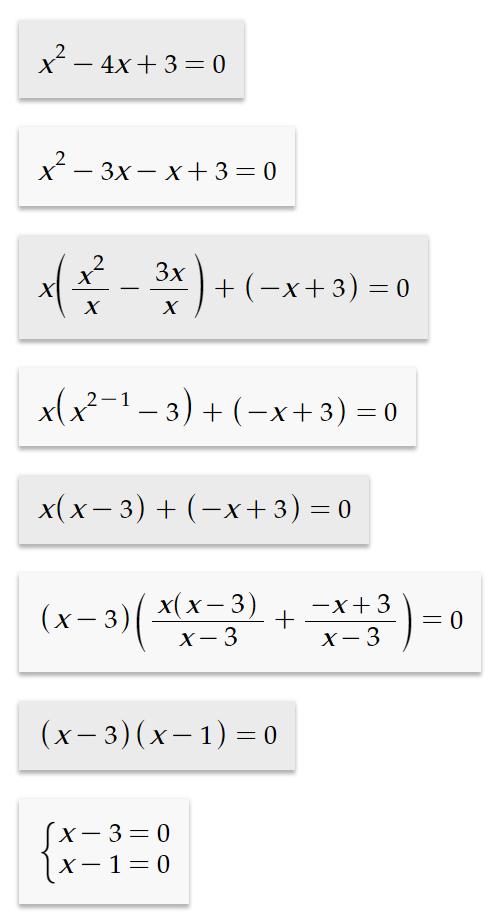
\includegraphics[width=0.5\linewidth]{quickmath4}
	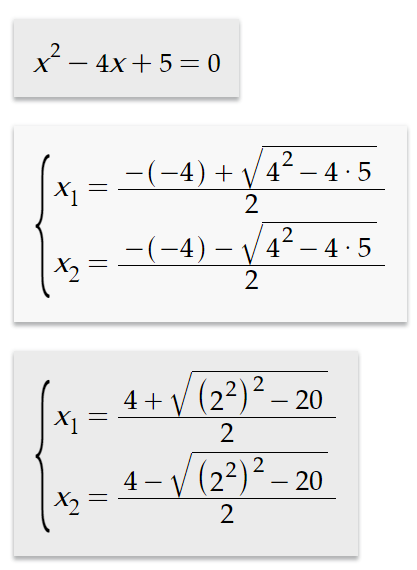
\includegraphics[width=0.5\linewidth]{quickmath5}
	\caption{Giải phương trình bậc hai trong \textbf{QuickMath}}
	\label{fig:quickmath4}
\end{figure}
\item Các tri thức về giải tích khá đầy đủ và bổ trợ cho nhau, \textbf{QuickMath} có thể tính đạo hàm từng phần, vi phân, tích phân của các hàm số và cả hàm lượng giác; vẽ đồ thị của nhiều hàm số lên cùng 1 trục tọa độ. Bên cạnh đó, ứng dụng còn có thể tính tích phân bội.
\begin{figure}
	\centering
	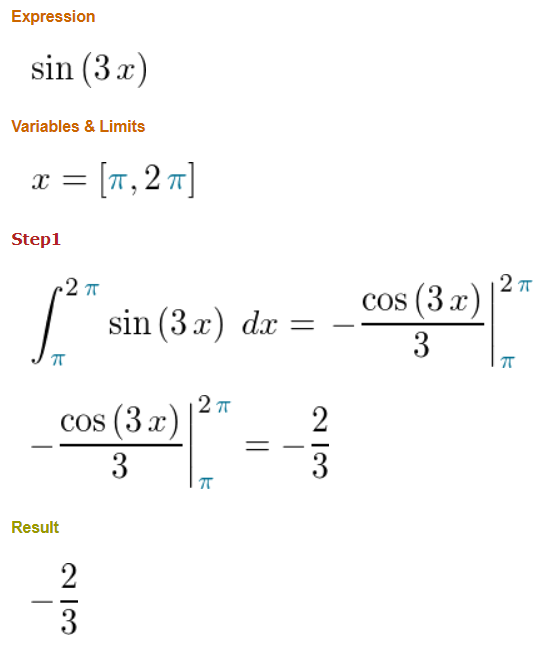
\includegraphics[width=0.5\linewidth]{quickmath6}
	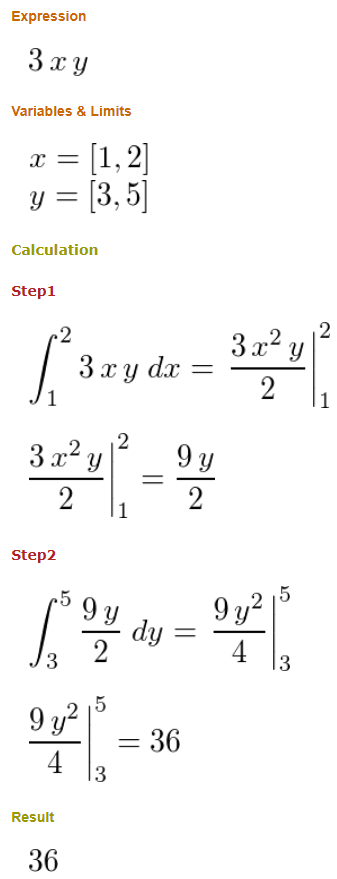
\includegraphics[width=0.5\linewidth]{quickmath7}
	\caption{Tính tích phân trong \textbf{QuickMath}}
	\label{fig:quickmath6}
\end{figure}
% \item Các phương pháp biểu diễn tri thức tạo ra trong hệ thống chưa bao quát được hết những trường hợp trong thực tế, do đó ứng dụng chỉ có thể giải quyết những bài toán đơn giản, chưa giải quyết được những bài toán phức tạp đòi hỏi những phép biến đổi, suy luận phức tạp.
\end{itemize}

\end{enumerate}	

\end{document}